\documentclass{ctexart}
\usepackage[utf8]{inputenc}
\title{TITLE}
\author{NAME}
\date{DATE}

\usepackage{natbib}
\usepackage{graphicx}
\usepackage{amsmath}
\usepackage{amssymb} 
\usepackage{amsthm}
\usepackage{mathtools}
\usepackage{xcolor}
\usepackage{bbm}
\usepackage{tocloft}
\usepackage{enumitem}
\usepackage{tikz}
\usepackage{hyperref}

\usepackage{url}
\usepackage[title]{appendix}
\usepackage{subcaption}

\usepackage[T1]{fontenc}
\usepackage{listings}
\usepackage[scaled]{beramono}


\lstset{%
  basicstyle=\ttfamily
  %showstringspaces=false,
  %tabsize=2,
  %upquote=true,
  %columns=fixed,
}

\DeclarePairedDelimiter\abs{\lvert}{\rvert}
\DeclarePairedDelimiter\norm{\lVert}{\rVert}

\DeclareGraphicsExtensions{.pdf}
\parindent 0cm
\parskip 0.2cm
\topmargin 0.2cm
\oddsidemargin 1cm
\evensidemargin 0.5cm
\textwidth 15cm
\textheight 21cm
\setlength{\unitlength}{0.7cm}
\thicklines

\theoremstyle{definition}

\newtheorem{theorem}{Theorem}[section]
\newtheorem{example}{Theorem}[section]
\newtheorem{proposition}[theorem]{Proposition}
\newtheorem{corollary}[theorem]{Corollary}
\newtheorem{lemma}[theorem]{Lemma}
\newtheorem{remark}[theorem]{Remark}
\newtheorem{definition}[theorem]{Definition}
\let\example\relax
\newtheorem{example}[theorem]{Example}
\newtheorem{algorithm}[theorem]{Algorithm}

\DeclareMathOperator{\GL}{GL}
\DeclareMathOperator{\trace}{tr}
\DeclareMathOperator{\id}{id}
\DeclareMathOperator{\op}{op}
\DeclareMathOperator{\lcm}{lcm}
\DeclareMathOperator{\hcf}{hcf}
\DeclareMathOperator{\im}{Im}

\newcommand{\gen}[1]{\langle #1 \rangle}

\newcommand{\todo}{\textcolor{red}{todo:}}

\newcommand{\N}{\mathbb{N}}
\newcommand{\Z}{\mathbb{Z}}
\newcommand{\R}{\mathbb{R}}
\newcommand{\F}{\mathbb{F}}
\newcommand{\Q}{\mathbb{Q}}
\newcommand{\finf}[1]{\F_#1}

\newcommand{\normalof}{\trianglelefteq}
\newcommand{\quot}[2]{{^{\textstyle #1}\big/_{\textstyle #2}}}
\newcommand{\homsig}{\phi : G \rightarrow H}
\newcommand{\CF}[2]{\Tilde{#1}(\mathbb{F}_{#2})}
\renewcommand{\O}{\mathcal{O}}

\newcommand{\forwarddir}{$( \Rightarrow )$}
\newcommand{\backwarddir}{$( \Leftarrow )$}
\setlength{\parindent}{2em}
\setlength{\parskip}{0.5em}

\title{在什么时候，我们该在酒馆战棋中选择芬利\\
When do we want Finley, and how often？}
\author{小弦切切 }
\date{2020-12-16}

\begin{document}
\maketitle
\newpage
\begin{figure}
    \centering
    
\includegraphics[width=0.3\textwidth, height=0.3\textheight]{pics/finley portrait.png}
    \caption*{冒险，出发！}
    \label{fig:my_label}
\end{figure}

\section*{序}
事实上，作者本人也没搞明白为什么这么个摸鱼文章要这么正经的写一个序。这个小短文的主要目的是探究一下芬利·莫格顿爵士在炉石酒馆战棋中的抓位，从而得到“当我看到我的其他英雄选择有多差时，我就可以选芬利重新洗牌了”的结论。作者本人在概率和统计方面的知识并不充沛，这可能也算是作者自己的一次小冒险吧，那么，出发！
\begin{flushright}
作者 \ 小弦切切 \\
2020年12月16日晚，在家里
\end{flushright}
\newpage
\tableofcontents
\newpage
\section{背景介绍}
芬利·莫格顿爵士并不在酒馆战棋的首发英雄之列，但在2019年11月19日也加入到游戏当中。然而，由于其技能“力量强化”过于不堪，芬利在2020年1月被请出酒馆回“炉”重做。

两个月后，芬利于3月17日回归，技能变成了如今我们熟悉的“冒险出发！”。虽然由于其他英雄的影响，芬利在2020年11月5日被短暂移除，不过在“奥秘哥”伟大的阿克扎曼兹拉克的问题被解决，芬利爵士也在12月15日的补丁中再度回归。在接下来的讨论中，我们默认芬利爵士为带有“冒险出发！”的技能。
\begin{figure}
    \centering
    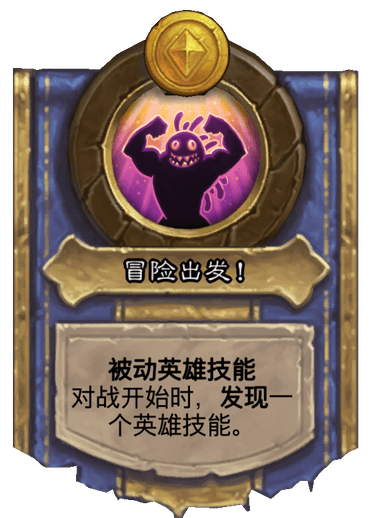
\includegraphics[width=0.3\textwidth, height=0.3\textheight]{pics/finley heropower.png}
    \caption*{小知识：芬利的两个技能使用的是同一张贴图，然而惊人的都不违和}
    \label{fig:my_label}
\end{figure}

这个技能决定了芬利成为了大多数对局中的备胎。只有我们见到其他英雄不怎理想时，我们才会选择芬利爵士，尝试获得一个更好的技能。发现的机制则是确保这个技能能带给我们正向收益的关键，因为玩家可以自行选择最强的技能。

那么，在什么时候我们应当选择芬利而非其他已经有确定技能的英雄呢？随机出来的三个技能中最强的那个的强度期望是多少？这便是作者想要探讨的“芬利问题”。
\section{假设和模型的建成}
接下来我们尝试将这个问题的数学部分提取出来进行分析。
\subsection{对于其他英雄技能的假设}
在每个对局中，英雄技能的强度是可比较的，允许从最强到最弱进行排序。这样我们可以将其他在池中的$n$个英雄技能描述为$\{1,2,3...n\}$,最强的英雄技能标注为1，第二强的英雄技能标注为2，以此类推最弱的英雄技能标注为$n$。

值得注意的是，不同种族池的英雄并不相同，这意味这在不同对局中，$n$值并不固定，\footnote{例如帕奇斯绑定海盗出现，红龙、伊瑟拉绑定龙族，奇恩瓦拉绑定元素等}且对于一个特定英雄，不同种族池对应的数字并不一定相同。\footnote{例如“女巴”詹迪斯·巴罗夫，没有野兽和鱼人会极大降低这个技能的强度。}

\subsection{对于芬利技能的假设}
\begin{itemize}
    \item 芬利不会提供相同的发现项，三个技能互不相同。
    \item 芬利仅会发现在本局对战池中的技能，例如在没有龙的对局当中，芬利不会提供红龙阿莱克斯塔萨的“红龙女王”技能
    \item 芬利发现的技能与对战中其他玩家选择的角色无关，被其他玩家选择的技能也会出现。例如一个对战中会出现有两个至尊盗王拉法姆的技能“归我了！”。
    \item 芬利是随机发现技能的，霉比/欧皇请不要硬黑/吹芬利只给垃圾/无敌技能。
\end{itemize}

\subsection{对于玩家的假设}
\begin{itemize}
    \item 玩家积极上进（是铁分奴），都选最强的技能。（不像作者看到阿凯就走不动路）
    \item 玩家没有不熟练/不会的技能以确保所有技能都能发挥出应有的表现。（不像作者到现在都玩不明白两个巴罗夫）
\end{itemize}
基于如上假设，作者提出芬利问题如下。\\
{\bfseries \emph{Finley Problem 芬利问题：}}固定$n > 3 $,考虑集合$S_n=\{1,2,...n\}$,从$S_n$中随机抽取不相同的三个数字$x_1,x_2,x_3 \in S_n$。求变量$F_n=min\{x_1,x_2,x_3\}$的期望$E(F_n)$。
\section{对于芬利问题的初步分析}
首先我们对这个问题进行一些直观的了解，得到一些定性的结论，为之后严谨的计算提供一些直觉。这部分的内容也是作者在思考到这个问题之后最先想到的一些点。
\subsection{期望的下限以及变量的下限}
\begin{itemize}
    \item 如果我们在数字1到$n$当中随机选择，那么我们的期望是这些数字的平均数$\frac{1+n}{2}$。因此当$n$是一个不大的整数时\footnote{此处指$n$不趋近于无穷大}，$E(F_n) < \frac{1+n}{2}$
    \item 由于我们从三个数字中选择最小值，则一定有$F_n < n,n-1$。而在最差（霉比）的情况下，$F_n=n-2$。因此$F_n \leq n-2$
\end{itemize}
\subsection{小n值时的情况}
\begin{itemize}
    \item $n=3$:此时$F_3==1 \Rightarrow E(F_3)=1$
    \item $n=4:\binom{4}{3}=4$,所以共有如下四种情况：
    \begin{center}
 \begin{tabular}{||c |c||} 
 \hline
 $\{x_1,x_2,x_3\}$ & $F_4$ \\ [0.5ex] 
 \hline\hline
 {1,2,3} & 1  \\ 
 \hline
 {1,2,4} & 1 \\
 \hline
 {1,3,4} & 1\\
 \hline
 {2,3,4} & 2 \\
 \hline
\end{tabular}
\end{center}
我们得到$E(F_4)=1.25$
\item $n=5: \binom{5}{3}=10$,我们进行最后一次穷举：
    \begin{center}
 \begin{tabular}{||c |c|| c | c ||} 
 \hline
 $\{x_1,x_2,x_3\}$ & $F_5$ & $\{x_1,x_2,x_3\}$ & $F_5$\\ [0.5ex] 
 \hline\hline
 {1,2,3} & 1 & {1,4,5} & 1\\ 
 \hline
 {1,2,4} & 1 & {2,3,4} & 2\\
 \hline
 {1,2,5} & 1 & {2,3,5} & 2\\
 \hline
 {1,3,4} & 1 & {2,4,5} & 2\\
 \hline
 {1,3,5} & 1 & {3,4,5} & 3\\
 \hline
\end{tabular}
\end{center}
得到$E(F_5)=1.5$
\end{itemize}
\section{对于芬利问题的进一步分析}
\subsection{从代码中获得数值解}
接下来作者打算借助代码的帮助，然而在上手之后发现这个问题在Matlab中犹如热刀切黄油一样游刃有余。作者对于在数学部分分析的无力以及编程部分过于轻松而同时深感沮丧，不过还是把一些小小的发现分享出来。

首先，Matlab中有内置的二次系数的计算方程$nchoosek(n,k)$,$n,k$为整数。其次，当$k$是一个数列时，方程输出这个数列中取$k$个元素的所有情况的矩阵。{\bfseries 并且，}这个矩阵已经贴心的从小到大排列好了，也就是说，每一行的最小值就是第一列的值。

再然后，这个问题就解决了...

\begin{figure}
    \centering
    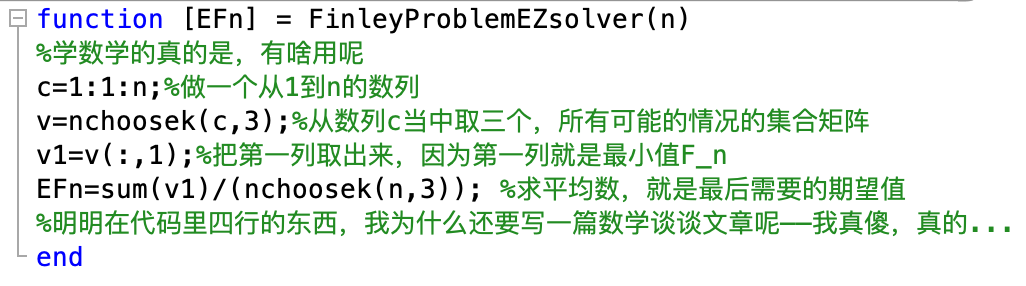
\includegraphics[ width=1.1\textwidth, height=0.2\textheight]{pics/code.png}
    \caption*{数学系废物自闭了，真的}
    \label{fig:my_label}
\end{figure}
\section{结论}

\subsection{纯粹数学问题的结论}
主要来关注一下这个值在$n$值增大并趋近于无穷时的表现：需要承认，作者一开始的想法是这个值会趋近于0.5，然而作者的理解可能不太行。
\begin{figure}[h]
    \centering
    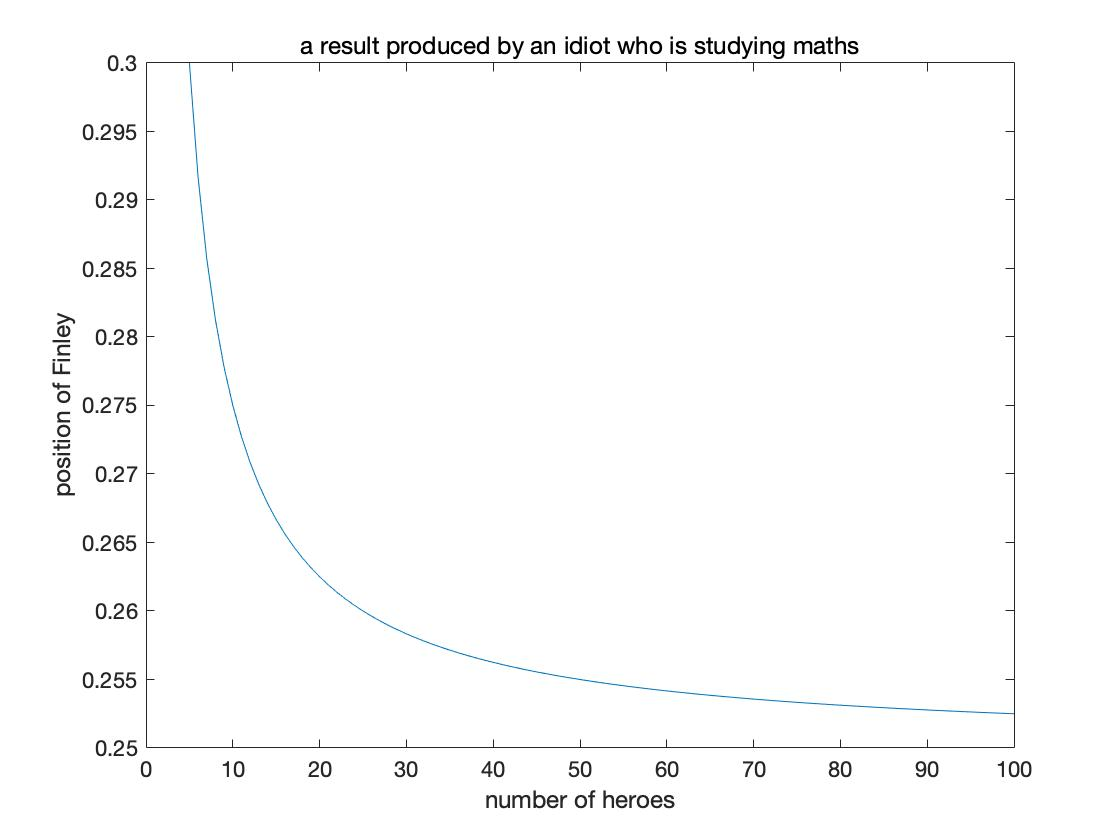
\includegraphics[width=0.7\textwidth, height=0.3\textheight]{pics/result.jpg}
    \caption*{这个曲线是从横坐标=5开始的}
    \label{fig:my_label}
\end{figure}
可以看出这个数据还是比较稳定的，并且在$n$值增大后，开始向0.25趋近。
\subsection{对于游戏内的结论}
在我们的模型之下，芬利的排名会稳定在所有英雄的前百分之二十五左右。因此芬利的强度取决于酒馆当中英雄的数量。版本更新后，除芬利外的英雄数量是51个，因此我们可以大约把芬利理解为一个胜率排名12-13位的英雄。

新版本更新不久所以没有大数据统计，这里我引用@塞戈德12月12日在bilibili发布的数据。当时英雄池总量是48个。如果有芬利在场上，那么他的英雄强度排名会在12位左右，在他之前的值得选的十一个英雄技能和强度如下：
\begin{center}
    
\begin{tabular}{||c|c||c|c||}
     \hline
     中位数分段（5800+）& 平均成绩& 前百分之一分段（12000+）&平均成绩  \\
     \hline
    迦拉客隆 & 3.84 & 迦拉客隆 & 3.86\\
         \hline
    伊利斯·逐星 & 3。91 & 伊利斯·逐星 & 3.90\\
         \hline
    拉格纳罗斯 & 4.17 & 马维·影歌 & 4.19\\
         \hline
    奥拉基尔 & 4.18 & 乔治 & 4.20\\
         \hline
    树人欧穆 & 4.25 & 米尔豪斯 & 4.21\\
         \hline
    乔治 & 4.27 & 小鱼人 & 4.21\\
         \hline
    巫妖王 & 4.29 & 拉法姆 & 4.22\\
         \hline
    米尔豪斯 & 4.30 & 拉格纳罗斯 & 4.24\\
         \hline
    拉法姆 & 4.31 & 詹迪斯·巴罗夫 & 4.26\\
         \hline
     马维·影歌 & 4.34 & 巫妖王 & 4.34\\
         \hline
    米尔菲斯 & 4.40 & 树人欧穆 & 4.38\\
         \hline
    {\bfseries 可能的芬利} & 4.42 & {\bfseries 可能的芬利} & 4.41\\
         \hline
\end{tabular}
\end{center}
总结来说，当开局的英雄选择中没有出现上述英雄的时候，我们可以选择芬利，并且期望给我们一个能排进前十强度的技能。不管是在中位数分段还是高分段，芬利都排在T2中流，是扎实的烂分英雄。然而版本上线首日大数据，芬利平均成绩仅有4.59，与本文预期相差较大。作者认为可能现在大家还在“尝鲜”阶段，等到环境稳定，芬利就会成为稳定的强力英雄了
\section*{作者想说的一些话}
写到这的时候，作者内心是五味杂陈，五谷杂粮，五谷丰登的。

数学系学生自主摸鱼探索的问题最后由简单的四行代码解决，内心的纠结是堪比当面NTR的。这也提醒了我以后在处理日常问题的时候，还是要从效率与实际出发，很多时候过于理想的去思考一个数学问题，对于实际生活的帮助，以及处理问题的效率都会有所影响。哎这么说好心酸啊，不过一味追求analytical solution确实在短期看更像是数学家的自我满足而非对社会作出的贡献。想不明白为什么我会学数学了...但凡我Matlab熟悉一点，都不至于花上一整晚的时间折腾这么点简单的东西。引以为戒，引以为戒。

关于炉石游戏，最近的负面情绪可能更多。我和同学平时聊天联机搓炉石的时候聊近期的游戏改动也是固定话题。其中战令也聊了不少。老实讲最近的炉石本身带给我的快乐既低级又匮乏，更多时候是以一个社交内容伴随着我。

所以我想聊聊那个让我开心的炉石。那也是公认的炉石巅峰时段（之一），2016年的上半段，探险者协会发布。探险者协会给炉石留下了三大宝贵遗产：探险者协会五人组的IP（我们把可爱的反派也算上）；宇宙机制初亮相；以及最重要的，成为了炉石永恒词条的发现。发现机制确实是对炉石随机性最好的体现，随机之后的可控部分妙在何处想必不用我再说，大家应该都有过惊奇秒拿奠定胜局，或者是三个垃圾纠结难选反复“撒币”的体验。当时作者刚上初三准备中考，而且我还是初三换了个班读的书，所以那时玩的炉石也成为了我和新同学快速了解，以及忙里偷闲高危玩手机的用途。不过作者中考考砸了这个是后话。

之后的炉石当然很精彩，只不过对我而言没有什么更值得称道的内容了。玩还是玩到了现在，但更像是打卡签到，而非真正从这游戏中获得些什么更多的快乐。阈值在一开始就被捅到天花板了。

说来也巧，去年夏天之前我afk了两个月，也是我最近这五年唯一afk的时间，最后也是看到暴雪炒起了究极冷饭奥丹姆，看到探险者协会四人组，听到五年前的那个主题曲片段，一上头就回来开了60包。那个有点西部牛仔味的主题曲，就等价于我心中最美好的炉石。

最近为了写一篇另外的战令文章看了不少社区里的观点，营地和Reddit刷的我实在有点负面情绪爆炸。不过我也不打算发表我的观点，打算写的文章也没动工就决定停了，当个对世界没有影响的观察者也挺好。如果炉石真的不但没有带给你快乐，那又何必像个忠贞的老实人一样坚守呢？我发誓我去年afk的两个月是我去年最快乐的时光，afk之后的炉石也带给了我比以往更多的快乐。

最后还是打算吹一吹芬利和发现词条，祝大家玩快攻能发现直伤，玩low比卡组能发现解场和回复，玩otk不被对面的发现恶心到，玩奥秘哥能发现冰箱，玩红龙能发现卡雷。炉石和生活都会迎来一场华丽的冒险，即使前路充满随机和未知，我们依旧选择冒险出发！
“哒哒哒～哒哒哒哒～等等～等等～等哒哒哒啦哒～”
\end{document}
